\documentclass{standalone}
\usepackage{pgfplots}
\pgfplotsset{compat=1.18}
\usepackage{amsmath}
\usepackage{tikz}
\usepackage{xcolor}
\usetikzlibrary{arrows.meta, positioning, calc}

\definecolor{noiseBlue}{HTML}{1565c0}
\definecolor{envOrange}{HTML}{e65100}
\definecolor{finalGreen}{HTML}{2e7d32}
\definecolor{toneBlue}{HTML}{1a6eb5}

\begin{document}
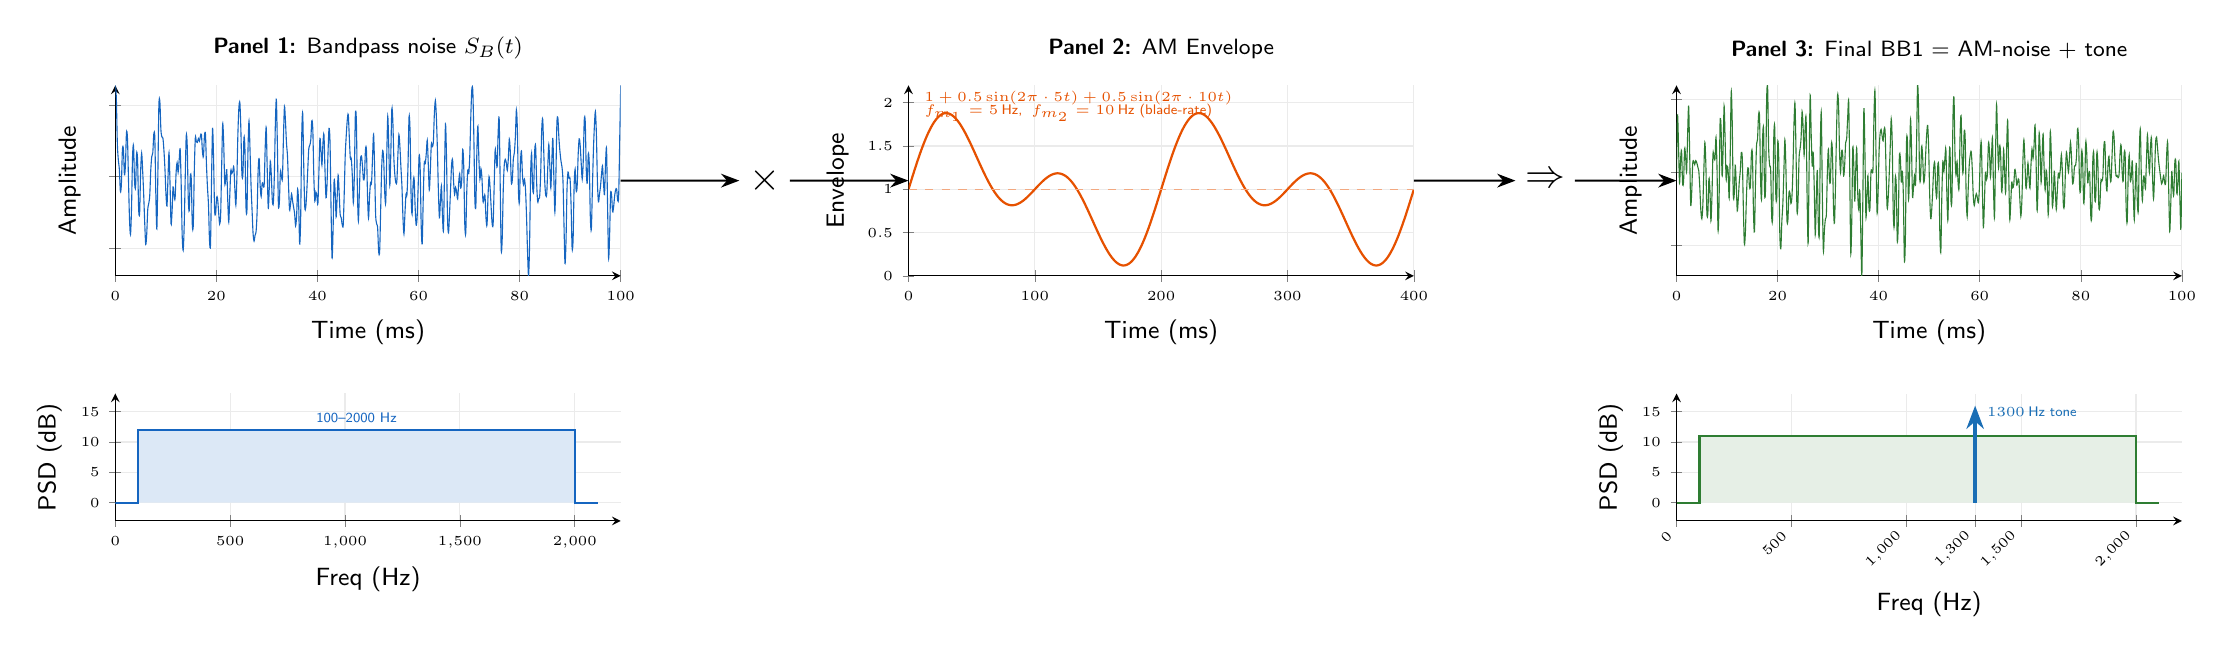
\begin{tikzpicture}[>=Stealth, font=\sffamily\small]

%% ── PANEL 1: Bandpass noise (time + PSD) ────────────────────────────────
\begin{axis}[
  name=p1time,
  at={(0,0)},
  width=8cm, height=4cm,
  xmin=0, xmax=100,
  ylabel={Amplitude}, xlabel={Time (ms)},
  title={\footnotesize\textbf{Panel 1:} Bandpass noise $S_B(t)$},
  yticklabels={}, grid=both, grid style={black!8},
  axis lines=left,
  tick label style={font=\sffamily\tiny},
  title style={font=\sffamily\footnotesize}
]
  %% Pseudo-noise: sum of many random sinusoids in 100-2000 Hz band
  \addplot[noiseBlue, thin, smooth, samples=500, domain=0:100]
      { 0.6*sin(deg(2*pi*0.13*x + 0.5))
       +0.5*sin(deg(2*pi*0.24*x + 1.2))
       +0.4*sin(deg(2*pi*0.41*x + 2.1))
       +0.7*sin(deg(2*pi*0.57*x + 0.8))
       +0.3*sin(deg(2*pi*0.78*x + 1.7))
       +0.5*sin(deg(2*pi*0.95*x + 0.3))
       +0.4*sin(deg(2*pi*1.13*x + 2.5))
       +0.3*sin(deg(2*pi*1.41*x + 1.1))};
\end{axis}

\begin{axis}[
  name=p1psd,
  at={(p1time.below south west)}, anchor=above north west, yshift=-0.5cm,
  width=8cm, height=3.2cm,
  xmin=0, xmax=2200, ymin=-3, ymax=18,
  ylabel={PSD (dB)}, xlabel={Freq (Hz)},
  grid=both, grid style={black!8}, axis lines=left,
  tick label style={font=\sffamily\tiny},
  xtick={0,500,1000,1500,2000},
]
  %% Bandpass rectangle 100-2000 Hz
  \addplot[noiseBlue, thick, fill=noiseBlue!15] coordinates
      {(0,0)(100,0)(100,12)(2000,12)(2000,0)(2100,0)};
  \node[noiseBlue, font=\sffamily\tiny] at (axis cs:1050, 14)
      {100--2000 Hz};
\end{axis}

%% ── PANEL 2: AM Envelope ────────────────────────────────────────────────
\begin{axis}[
  name=p2,
  at={(p1time.right of north east)}, anchor=left of north west,
  xshift=2.2cm,
  width=8cm, height=4cm,
  xmin=0, xmax=400,
  ymin=0, ymax=2.2,
  ylabel={Envelope}, xlabel={Time (ms)},
  title={\footnotesize\textbf{Panel 2:} AM Envelope},
  grid=both, grid style={black!8}, axis lines=left,
  tick label style={font=\sffamily\tiny},
  title style={font=\sffamily\footnotesize}
]
  %% envelope = 1 + 0.5*sin(2*pi*5e-3*t) + 0.5*sin(2*pi*10e-3*t)
  %% t in ms -> 5 Hz = 0.005 cycles/ms; 10 Hz = 0.01 cycles/ms
  \addplot[envOrange, thick, smooth, samples=400, domain=0:400]
      {1 + 0.5*sin(deg(2*pi*0.005*x)) + 0.5*sin(deg(2*pi*0.01*x))};
  \draw[envOrange!50, dashed, thin] (axis cs:0,1) -- (axis cs:400,1)
      node[right, font=\sffamily\tiny, envOrange]{baseline};
  \node[envOrange, anchor=west, font=\sffamily\tiny] at (axis cs:5, 2.05)
      {$1 + 0.5\sin(2\pi\cdot5t) + 0.5\sin(2\pi\cdot10t)$};
  \node[envOrange, anchor=west, font=\sffamily\tiny] at (axis cs:5, 1.88)
      {$f_{m_1}=5\,\text{Hz}$,\; $f_{m_2}=10\,\text{Hz}$ (blade-rate)};
\end{axis}

%% ── PANEL 3: Final BB1 waveform ─────────────────────────────────────────
\begin{axis}[
  name=p3time,
  at={(p2.right of north east)}, anchor=left of north west,
  xshift=2.2cm,
  width=8cm, height=4cm,
  xmin=0, xmax=100,
  ylabel={Amplitude}, xlabel={Time (ms)},
  title={\footnotesize\textbf{Panel 3:} Final BB1 = AM-noise + tone},
  yticklabels={}, grid=both, grid style={black!8},
  axis lines=left,
  tick label style={font=\sffamily\tiny},
  title style={font=\sffamily\footnotesize}
]
  %% AM-modulated noise approximation + tone at 1.3 cycles/ms
  \addplot[finalGreen, thin, smooth, samples=500, domain=0:100]
      { (1 + 0.5*sin(deg(2*pi*0.005*x)) + 0.5*sin(deg(2*pi*0.01*x))) *
        (0.4*sin(deg(2*pi*0.13*x))+0.5*sin(deg(2*pi*0.57*x))
        +0.4*sin(deg(2*pi*0.95*x))+0.3*sin(deg(2*pi*1.41*x)))
       + 0.5*sin(deg(2*pi*1.3*x)) };
\end{axis}

\begin{axis}[
  name=p3psd,
  at={(p3time.below south west)}, anchor=above north west, yshift=-0.5cm,
  width=8cm, height=3.2cm,
  xmin=0, xmax=2200, ymin=-3, ymax=18,
  ylabel={PSD (dB)}, xlabel={Freq (Hz)},
  grid=both, grid style={black!8}, axis lines=left,
  tick label style={font=\sffamily\tiny},
  xtick={0,500,1000,1300,1500,2000},
  xticklabel style={rotate=45, anchor=east, font=\sffamily\tiny},
]
  %% Broadband plateau
  \addplot[finalGreen, thick, fill=finalGreen!12] coordinates
      {(0,0)(100,0)(100,11)(2000,11)(2000,0)(2100,0)};
  %% Tone spike at 1300 Hz
  \addplot[toneBlue, very thick, ->]
      coordinates {(1300, 0) (1300, 16)};
  \node[toneBlue, font=\sffamily\tiny, anchor=west]
      at (axis cs:1310, 15) {$1300\,\text{Hz}$ tone};
\end{axis}

%% ── Operator arrows between panels ─────────────────────────────────────
% Arrow + × symbol between Panel 1 and Panel 2
\node[font=\Large] (times12) at
    ($(p1time.east)!0.5!(p2.west)$) {$\times$};
\draw[->, thick] (p1time.east) -- (times12.west);
\draw[->, thick] (times12.east) -- (p2.west);

% Arrow + = symbol between Panel 2 and Panel 3
\node[font=\Large] (eq23) at
    ($(p2.east)!0.5!(p3time.west)$) {$\Rightarrow$};
\draw[->, thick] (p2.east) -- (eq23.west);
\draw[->, thick] (eq23.east) -- (p3time.west);

\end{tikzpicture}
\end{document}
